\subsection{Servomoteurs}

Les fonctions de commande liées au déploiement des aérofreins et à l’actionnement des mécanismes du lanceur SP-02 reposent sur
l’utilisation de servomoteurs. Le choix de ces actionneurs conditionne directement l’architecture d’alimentation, la précision
de commande et la robustesse globale du système.\\

\begin{minipage}{0.3\textwidth}
    \centering
    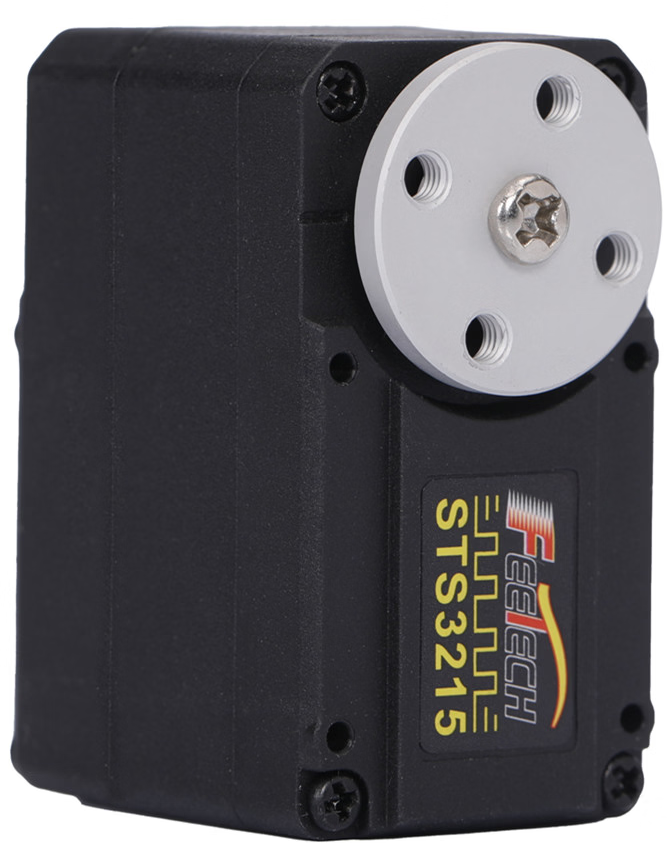
\includegraphics[width=\textwidth]{figures/Sts3215.png}
    \captionof{figure}{Servomoteur STS3215}
    \label{fig:sts3215}
\end{minipage}
\hfill
\begin{minipage}{0.65\textwidth}
    Les servomoteurs STS3215 ont été retenus comme un compromis adapté aux besoins du projet en termes de coût, de couple
    disponible et de capacités de contrôle. Leur couple maximal de 19,5 kg.cm offre une marge confortable vis-à-vis des efforts
    attendus, tout en autorisant différents modes de fonctionnement.\\

    Les STS3215 intègrent une électronique de commande avancée incluant des capteurs internes de tension, de courant et de
    température, permettant la surveillance de leur état de fonctionnement et l’estimation indirecte du couple fourni et donc
    également du couple résistant. Cette fonctionnalité permet notamment de détecter les blocage. Par exemple, pour le cas des
    aérofreins, la détection d'un blocage lors de l'initialisation de la fusée permettrait de détecter la plage de déploiement
    minimal et maximal des aérofreins et donc d'étalonner le système.\\

    La communication s’effectue via une interface numérique de type Half-\acrshort{UART} \footnotemark basée sur
    des registres internes, les servomoteurs étant adressables et pouvant ainsi être chaînés sur une même ligne de communication.
\end{minipage}

\vspace{0.5cm}

Enfin, ces servomoteurs proposent plusieurs modes de fonctionnement, notamment un mode de contrôle en position basé sur un
encodeur magnétique multi-tours offrant une précision inférieure au degré, ainsi qu’un mode de contrôle en vitesse permettant
un fonctionnement en rotation continue. Cette polyvalence en fait une solution particulièrement adaptée aux exigences du projet.

\footnotetext{Le Half-\acrshort{UART} est une interface série asynchrone utilisant une seule ligne de données pour la
transmission et la réception de données.}

\newpage
